\section{Results}

\subsection{A frozen action-contrast transfer protocol}

The final experiment evaluated target offline adaptation using matched
counterfactuals from restored SUMO states (\Cref{fig:method-schematic}).  Target
roles were separated by seed, with seeds 5057 and 6067 reserved for adaptation.
Seed 8171 was collected after the joint method freeze for one offline
action-regret confirmation.  Seeds 8081 and 9091 were reserved for closed-loop
policy rollouts.  OOF models selected the blend; deployment used one refit per
external city on all valid adaptation groups.  Frozen artifact identities and
the regeneration contract are documented in
\Cref{sec:supp-artifact-chain,tab:artifact-chain}.

\begin{figure}[!htbp]
\centering
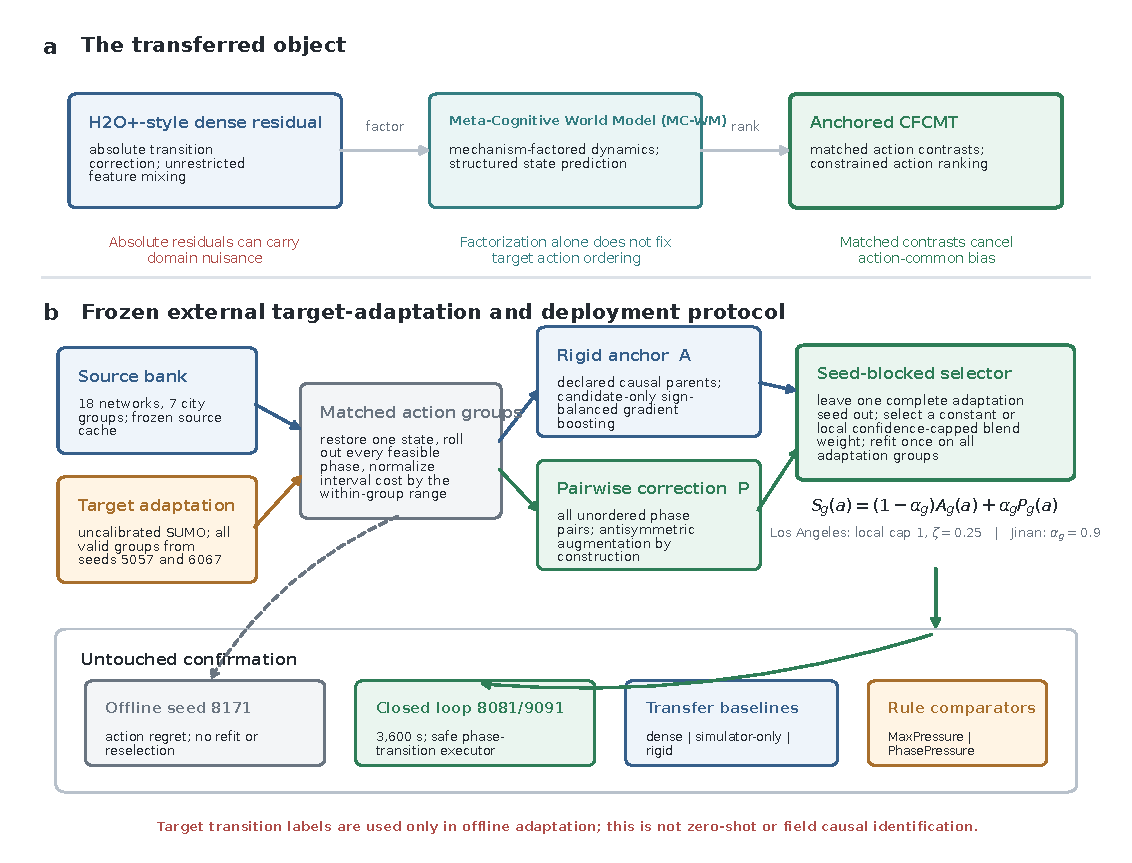
\includegraphics[width=\textwidth]{tsc_anchored_transfer_schematic.pdf}
\caption{Transferred object and frozen evaluation protocol. \textbf{a}, The
method lineage compares absolute dense-residual prediction and factored
Meta-Cognitive World Model (MC-WM) dynamics with the final matched-ranking
estimand.  The dense baseline in panel \textbf{b} uses the same matched contrast
data and target refit budget as CFCMT. \textbf{b}, A seed-blocked target selector
combines a rigid parent-restricted anchor with an antisymmetric all-pair
correction.  The pressure reference defines the contrast origin.  MaxPressure
and PhasePressure remain independent comparators, without serving as fallback
actions.  Target counterfactual labels make this a target offline adaptation
setting.}
\label{fig:method-schematic}
\end{figure}

The source bank comprised 18 networks in seven city groups: Atlanta, Cologne,
Hangzhou, Ingolstadt, New York, two RESCO synthetic grids and Salt Lake City.
Together, these networks contained 317 controlled traffic lights and 6,076
non-internal lanes.  The external set comprised a four-signal Los Angeles
corridor and a 12-signal Jinan grid with three demand files
(\Cref{fig:network-plate}; detailed counts in
\Cref{sec:supp-network-inventory,tab:network-scope}).
Development folds held out entire city groups to prevent related subnetworks
from entering training.  This excluded every Cologne, Hangzhou or Ingolstadt
subnetwork whenever its city was held out.

\begin{figure}[!htbp]
\centering
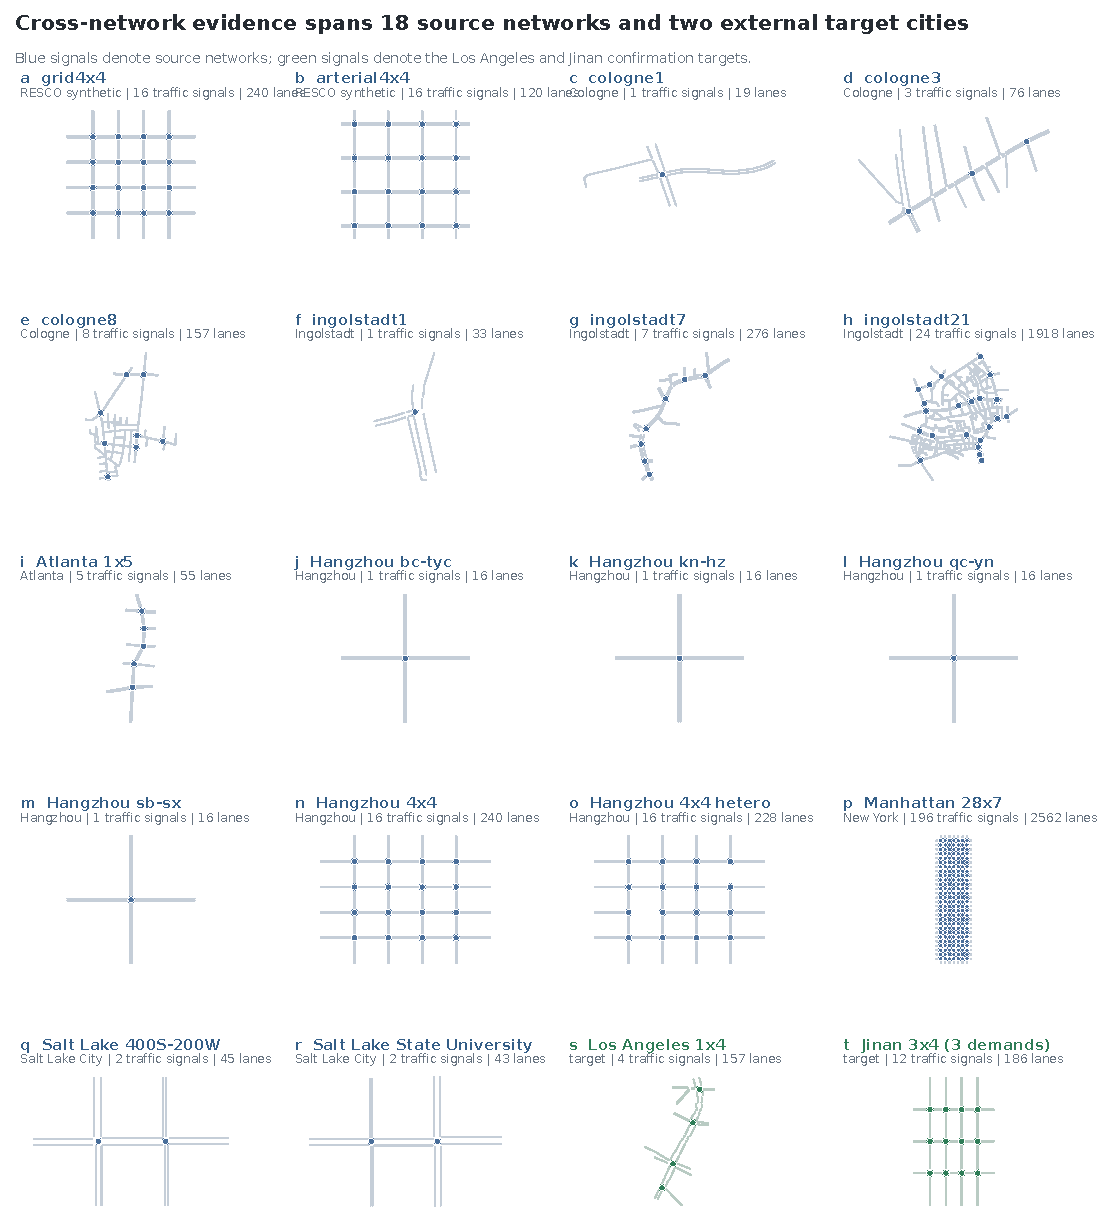
\includegraphics[width=\textwidth]{traffic_signal_transfer_networks.pdf}
\caption{Network shift in development and external confirmation.  Lines show
non-internal SUMO lanes, and points identify the controlled traffic lights.
Blue panels show 18 source networks grouped into seven development cities;
green panels show the external target geometries.  The Jinan geometry is paired
with three demand files for evaluation.  These converted networks document
topology and action-set variation without representing calibrated city-wide
digital twins.}
\label{fig:network-plate}
\end{figure}

\subsection{Seed-held-out development selected an action-contrast correction}

Models and the city-level selector were fitted on source seeds 2027 and 3037,
then evaluated on excluded seed 4047.  In leave-one-city-out evaluation,
city-macro normalized action regret fell from 0.2414 for the rigid anchor to
0.2177 for the selected anchored model.  This represented a 9.84\% reduction
across the seven held-out city groups (\Cref{tab:development-confirmation}).
Six groups improved; Hangzhou regressed by 0.00388, below the frozen 0.01
tolerance.

\begin{table}[t]
\caption{Seed-held-out development confirmation.  Regret is candidate cost
minus the matched-group optimum, normalized by the within-group action range;
lower is better.}
\label{tab:development-confirmation}
\centering
\small
\begin{tabular}{lrrr}
\toprule
Development result & Anchor regret & Selected regret & Relative gain \\
\midrule
Seven-city leave-one-city-out & 0.241 & 0.218 & 9.84\% \\
\bottomrule
\end{tabular}

\end{table}

Earlier variants failed their gates, which tested worst-city performance and
city-level stability.  A global pairwise correction regressed on the added
Salt Lake domain.  The first anchored selector exceeded its worst-city
tolerance, and a cross-fitted selector failed the city-level stability
requirement.  These outcomes were retained, and the successful seed-held-out
protocol was frozen before external labels were generated
(\Cref{sec:supp-development-history,tab:development-history}).

\subsection{External offline scores favoured source-plus-target fitting}

The external selector used all valid adaptation groups: 165 in Los Angeles and
911 across the three Jinan demands.  Holding out complete adaptation seeds
produced two selection folds for each city.  Los Angeles selected a local blend
with disagreement cap 1 and confidence multiplier 0.25.  Jinan selected a
constant correction weight of 0.9 across its demand files.  Each deployment
artifact was refitted once on all adaptation groups and frozen before seed
8171 was collected.

On seed 8171, Los Angeles regret decreased from 0.1482 to 0.1450 (2.18\%),
while optimal-action accuracy increased from 0.785 to 0.810.  Jinan regret
decreased from 0.4361 to 0.3921 (10.10\%), while accuracy increased from 0.296
to 0.342 (\Cref{tab:external-offline}; panel~\textbf{a} of
\Cref{fig:external-confirmation}).  With equal city weights, regret decreased
from 0.2922 to 0.2685 (8.09\%), with both city point estimates improving.

The freeze included a legacy near-target-only comparator from the same causal
action-advantage family.  It shared the feature semantics and target adaptation
groups, with a target prediction weight numerically equal to one.  Its deployed
weighted mean excluded source-labelled groups, although a retained source
prior could resolve exact action ties.  On seed 8171, this comparator achieved
regret 0.2172 in Los Angeles and 0.4036 in Jinan.  CFCMT reduced the equal-city
point estimate from 0.3104 to 0.2685 (13.48\%).

The paired action-group improvement over this comparator was 0.07219 in Los
Angeles (95\% interval $[0.01671,0.13512]$; two-sided bootstrap probability
value 0.011).  Jinan improved by 0.01150, with interval $[-0.02250,0.04524]$
and probability value 0.5196.  The offline advantage over the legacy comparator
was supported in Los Angeles and inconclusive in Jinan.

\begin{table}[t]
\caption{External seed-8171 offline confirmation after city-specific method
freeze.  The legacy near-target-only arm shares the causal action-ranking
family and target groups.  Its weighted mean has zero deployed source weight,
but exact ties retain a source prior.  Adaptation counterfactuals come from
seeds 5057 and 6067; held-out groups are excluded from fitting and selection.
Table gains compare CFCMT with the arm labelled target only.}
\label{tab:external-offline}
\centering
\scriptsize
\resizebox{\textwidth}{!}{\begin{tabular}{lrrrrrrr}
\toprule
City & Adaptation groups & Held-out groups & Anchor & Target only & CFCMT & CFCMT vs target only & Selected blend \\
\midrule
Los Angeles & 165 & 79 & 0.148 & 0.217 & 0.145 & 33.24\% & local cap 1, $\zeta=0.25$ \\
Jinan & 911 & 457 & 0.436 & 0.404 & 0.392 & 2.85\% & constant $\alpha_g=0.9$ \\
\midrule
External macro & -- & 2 cities & 0.292 & 0.310 & 0.269 & 13.48\% & city-specific \\
\bottomrule
\end{tabular}
}
\end{table}

Uncertainty in the comparison with the rigid anchor differed sharply between
the two cities.  A 10,000-replicate paired group bootstrap gave a Los Angeles
improvement interval of $[-0.0675,0.0729]$, with two-sided bootstrap probability
value 0.9396.  Jinan gave an interval of $[0.00469,0.08293]$ and probability
value 0.0274.  The Los Angeles point estimate therefore remained directional
with an interval spanning zero.  The predeclared external gate required at
least 2\% city-macro improvement, both cities improving and no city regression.
This engineering confirmation did not provide population-level inference
across target cities.

\begin{figure}[!htbp]
\centering
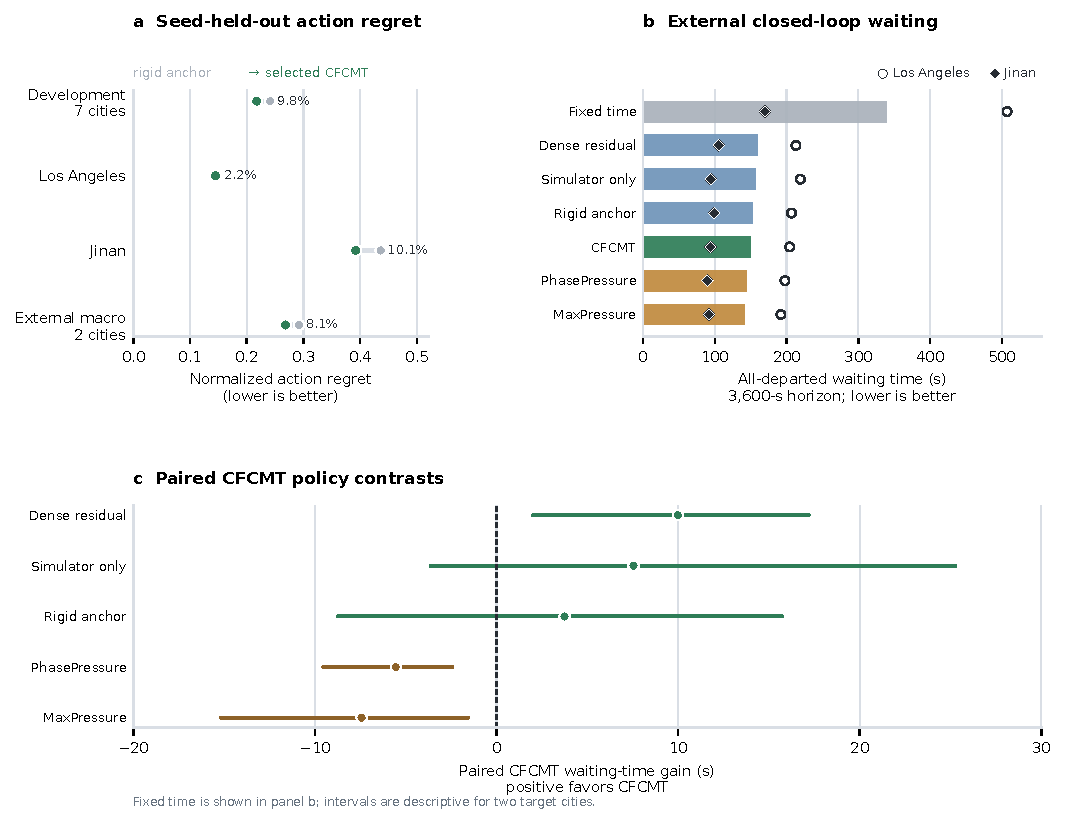
\includegraphics[width=\textwidth]{tsc_external_confirmation.pdf}
\caption{Original offline and seven-policy closed-loop confirmation. \textbf{a},
Seed-held-out normalized action regret for development cities and external
targets.  Green points show selected CFCMT scores, and grey points show the
rigid anchor. \textbf{b}, All-departed waiting by policy in Los Angeles
(circles) and Jinan (diamonds); bars show the equal-city macro.
\textbf{c}, Paired CFCMT gains in all-departed waiting relative to the non-fixed
comparators.  Fixed-time results remain visible in panel \textbf{b} and
\Cref{tab:external-closed-loop}.  Positive values favour CFCMT; intervals are
descriptive paired hierarchical bootstrap intervals for the original two-seed
matrix on two target cities.  The ten-new-seed confirmation is reported
separately in \Cref{fig:v43-dense-fresh10}.}
\label{fig:external-confirmation}
\end{figure}

\subsection{Matched action contrast reduced waiting relative to dense residual control}

The formal closed-loop matrix comprised four target scenarios, two seeds and
seven policies, yielding 56 completed 3,600-s rollouts.  The primary metric
measured mean waiting over all departed vehicles, including unfinished trips.
SUMO \texttt{write-unfinished} records accrued their waiting through the fixed
horizon.  Completed-only waiting, system vehicle-hours and completion were
reported alongside this metric to show censoring and throughput trade-offs.

Anchored CFCMT achieved 149.17 s all-departed waiting, compared with 159.15 s
for the H2O$^+$-style dense residual under the same information and refit
budget.  This reduction of 9.98 s (6.27\%) was observed in both Los Angeles
(8.46 s) and Jinan (11.50 s)
(\Cref{tab:external-closed-loop,sec:supp-city-outcomes,tab:external-city-results}).
The descriptive paired hierarchical bootstrap interval was $[2.01,17.19]$ s,
and 98.43\% of replicates favoured CFCMT.  Completed-only waiting also decreased
from 147.47 to 133.06 s in the same comparison.  System vehicle-hours decreased
from 618.15 to 594.14, and completion increased from 0.870 to 0.889.

Simulator-only control and the rigid anchor achieved 156.71 and 152.91 s
all-departed waiting, respectively.  CFCMT improved on their point estimates
by 7.54 s (4.81\%) and 3.75 s (2.45\%), respectively.  Both intervals crossed
zero, leaving the clearest closed-loop improvement against dense residual
transfer (\Cref{tab:external-comparisons}).  The anchor comparison was therefore
stronger in offline action regret than in closed-loop waiting.

\begin{table}[t]
\caption{Original two-seed, seven-policy external 3,600-s city-macro results.
Scenarios are
weighted equally within each city and the two cities are weighted equally.
Waiting times are seconds; system burden is vehicle-hours.  ``Incidents'' is
the equal-city mean of unique SUMO junction-collision incidents.}
\label{tab:external-closed-loop}
\centering
\scriptsize
\resizebox{\textwidth}{!}{\begin{tabular}{lrrrrrr}
\toprule
Policy & All-departed wait & Completed wait & System vehicle-hours & Unfinished & Completion & Incidents \\
\midrule
Fixed time & 338.58 & 308.72 & 885.18 & 0.133 & 0.661 & 2.00 \\
Dense residual & 159.15 & 147.47 & 618.15 & 0.066 & 0.870 & 0.25 \\
Simulator only & 156.71 & 138.68 & 619.66 & 0.069 & 0.877 & 0.00 \\
Rigid anchor & 152.91 & 138.40 & 606.30 & 0.072 & 0.882 & 0.50 \\
\textbf{Anchored CFCMT} & 149.17 & 133.06 & 594.14 & 0.067 & 0.889 & 0.00 \\
PhasePressure & 143.62 & 125.32 & 583.05 & 0.068 & 0.898 & 0.25 \\
MaxPressure & 141.74 & 135.42 & 580.29 & 0.065 & 0.896 & 0.25 \\
\bottomrule
\end{tabular}
}
\end{table}

\begin{table}[t]
\caption{Original two-seed CFCMT policy contrasts for all-departed waiting.  Positive
gains favour CFCMT.  Intervals are descriptive, not population-level city
inference.}
\label{tab:external-comparisons}
\centering
\scriptsize
\resizebox{\textwidth}{!}{\begin{tabular}{lrrrrr}
\toprule
Baseline & CFCMT gain (s) & Relative gain & Descriptive 95\% interval & Los Angeles gain & Jinan gain \\
\midrule
Fixed time & 189.42 & 55.94\% & [67.11, 308.32] & 302.90 & 75.93 \\
Dense residual & 9.98 & 6.27\% & [2.01, 17.19] & 8.46 & 11.50 \\
Simulator only & 7.54 & 4.81\% & [-3.62, 25.27] & 14.75 & 0.34 \\
Rigid anchor & 3.75 & 2.45\% & [-8.75, 15.70] & 2.36 & 5.14 \\
PhasePressure & -5.55 & -3.86\% & [-9.54, -2.45] & -6.91 & -4.19 \\
MaxPressure & -7.43 & -5.24\% & [-15.17, -1.56] & -12.53 & -2.33 \\
\bottomrule
\end{tabular}
}
\end{table}

\subsection{Ten new paired seeds confirmed the frozen dense-baseline advantage}
\label{sec:v43-dense-fresh10}

The frozen V43 CFCMT and dense models were next evaluated on ten new simulator
seeds across the same four scenarios.  The seed roster, primary comparison and
analysis were fixed before these outcomes were opened.  All 80 required
3,600-s rollouts completed with unchanged models, input networks, executor and
timing; no retraining, new target labels or parameter tuning occurred.

Equal-city all-departed waiting was 150.84 s for CFCMT and 158.67 s for dense,
a reduction of 7.83 s or 4.93\%
(\Cref{tab:v43-dense-fresh10,fig:v43-dense-fresh10}).  The preregistered paired
whole-seed bootstrap gave a CFCMT-minus-dense 95\% interval of
$[-11.85,-4.11]$ s; the corresponding relative reduction interval was
2.64--7.31\%.  Nine of ten equal-city seed contrasts improved.  Los Angeles
improved by 5.43 s on average, with six of ten seeds favourable; Jinan's
three-demand mean improved by 10.22 s, with all ten seeds favourable.
Completed-only waiting decreased from 147.49 to 132.88 s, system vehicle-hours
from 616.49 to 596.15, and completion increased from 87.59\% to 88.66\%.

The prespecified confirmation criterion was met: the primary mean difference
and its 95\% upper endpoint were below zero.  This new-seed result is reported
independently of the original 56-rollout matrix and the V91/V98 comparisons;
all ten seeds were retained.  The exact seed roster and unchanged execution
settings are given in \Cref{sec:methods-v43-dense-fresh10,sec:supp-v43-dense-fresh10}.

\begin{table}[t]
\caption{Independent ten-new-seed confirmation of the frozen V43 models.
Waiting includes every departed vehicle, including unfinished trips.
Jinan's three demands are weighted equally, followed by equal city and seed
weights.  Differences are CFCMT minus dense; negative waiting differences
favour CFCMT.  Seed counts refer to lower all-departed waiting, and secondary
outcomes use the same aggregation.  Completion differences are in percentage
points (pp).}
\label{tab:v43-dense-fresh10}
\centering
\small
\resizebox{\textwidth}{!}{\begin{tabular}{lrrrrr}
\toprule
Aggregation & \shortstack{CFCMT\\wait (s)} & \shortstack{Dense\\wait (s)} & \shortstack{Difference\\(s)} & \shortstack{Reduction\\(\%)} & \shortstack{Improved\\seeds} \\
\midrule
Equal-city mean & 150.84 & 158.67 & -7.83 & 4.93 & 9/10 \\
Los Angeles & 207.64 & 213.07 & -5.43 & 2.55 & 6/10 \\
Jinan & 94.05 & 104.27 & -10.22 & 9.80 & 10/10 \\
\midrule
\multicolumn{6}{l}{Secondary outcomes, equal-city means} \\
Metric & CFCMT & Dense & \multicolumn{3}{l}{Difference} \\
Completed-only wait (s) & 132.88 & 147.49 & \multicolumn{3}{l}{-14.61} \\
System vehicle-hours & 596.15 & 616.49 & \multicolumn{3}{l}{-20.34} \\
Completion (\%) & 88.66 & 87.59 & \multicolumn{3}{l}{+1.08 pp} \\
\bottomrule
\end{tabular}
}
\end{table}

\begin{figure}[!htbp]
\centering
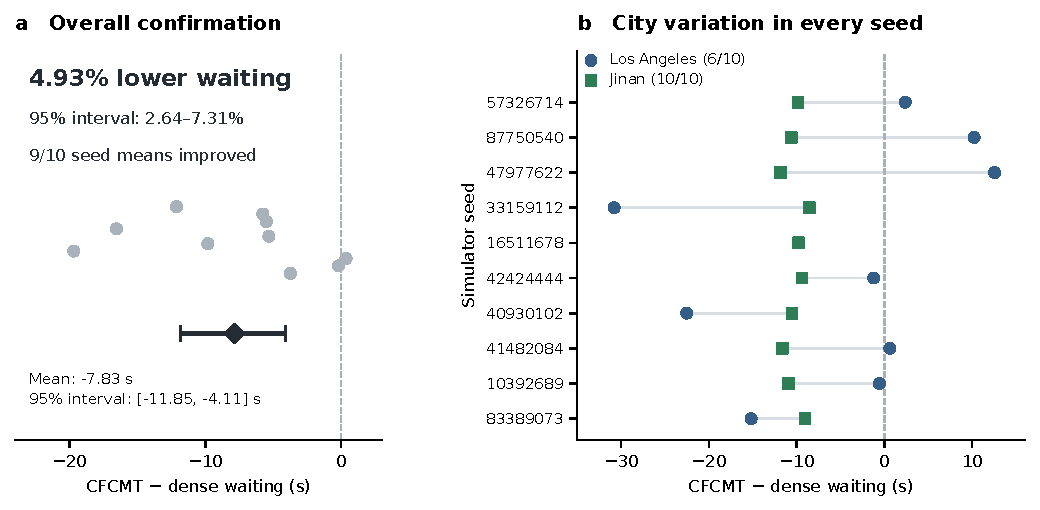
\includegraphics[width=\textwidth]{tsc_v43_dense_fresh10_confirmation.pdf}
\caption{Independent confirmation on ten new paired simulator seeds
(80 rollouts).  \textbf{a}, Grey points show equal-city CFCMT-minus-dense
waiting differences; vertical offsets aid visibility.  The diamond and
whiskers show the mean and registered 95\% percentile interval from 20,000
paired whole-seed-block bootstrap replicates, retaining both policies on all
four scenarios.  \textbf{b}, City-specific differences for the same ten seeds.
Negative values favour CFCMT.  Relative reduction is computed from the ratio
of macro means (\Cref{sec:methods-v43-dense-fresh10}); the interval describes
seed variation within the two fixed networks.}
\label{fig:v43-dense-fresh10}
\end{figure}

\FloatBarrier
\subsection{A fresh near-target-only comparison exposed network-dependent transfer}

The seven-policy V43 matrix omitted the frozen legacy near-target-only
comparator described in the offline evaluation.  We added it to the same
eight scenario--seed cells after observing the main outcomes.  This post-hoc
V90 ablation left both models unchanged, preserving the comparator's retained
source prior for exact ties.  CFCMT achieved 149.17 s city-macro all-departed
waiting, compared with 149.04 s for the comparator, a 0.12-s disadvantage.
Los Angeles favoured the comparator by 2.45 s, whereas Jinan favoured CFCMT by
2.20 s.  The post-hoc timing made this comparison descriptive rather than
confirmatory.

We then froze the V91 protocol before generating 64 further simulator seeds,
disjoint from all V43, V89 and V90 roles.  Each seed paired CFCMT with the legacy
comparator on Los Angeles and all three Jinan demands.  This produced 256
paired cells and 512 completed rollouts for the fresh confirmation.  The
primary relative difference averaged scenarios within city, weighted the two
cities equally within seed, then averaged seeds.  Negative values indicated
lower all-departed waiting for CFCMT than for the comparator.

The comparator achieved 149.09 s all-departed waiting, compared with 155.14 s
for CFCMT.  The equal-seed relative difference was $+4.254\%$ (paired 95\%
interval $[-0.775,13.211]\%$).  Only 29/64 seeds improved, with a one-sided
exact sign-test probability of 0.809.  City effects had opposite signs.
Jinan improved by 3.045\%, with all 64 seed-level city contrasts favouring
CFCMT.  Los Angeles regressed by 7.865\%, with improvement in 22/64 seed-level
city contrasts.

The worst seed regressed by 267.56\%; collision incidents totalled 25 for
CFCMT and 15 for the comparator.  Both policies completed all rollouts with
zero teleports in this confirmation.  The predeclared mean, interval,
both-city, worst-seed, improved-fraction, sign-test and collision gates did not
jointly pass.  Fresh source-contribution confirmation was rejected
(\Cref{tab:source-contribution}).  City and seed distributions
localized the rejection to the Los Angeles tail
(\Cref{fig:source-contribution-diagnostic,sec:supp-source-diagnostics}).

\begin{table}[t]
\caption{Closed-loop source-contribution ablation.  Both policies share target
adaptation groups, features, the action executor and target scenarios.  The
legacy comparator labelled ``target only'' has target weight numerically one
and retains a source prior for exact ties.  Positive differences denote higher
all-departed waiting for CFCMT relative to that comparator.  V90 is post-hoc;
V91 is the preregistered fresh-seed confirmation.  Incident entries report
CFCMT/target only counts for their respective evaluation matrices.}
\label{tab:source-contribution}
\centering
\scriptsize
\resizebox{\textwidth}{!}{\begin{tabular}{lrrrrrrrrr}
\toprule
Evidence & Seeds & Paired cells & Legacy near-target-only wait & CFCMT wait & CFCMT minus legacy wait & Los Angeles difference & Jinan difference & Improved & Incidents CFCMT/legacy \\
\midrule
V90 post-hoc & 2 & 8 & 149.04 & 149.17 & +0.082\% & +1.212\% & -2.292\% & 7/8 & 0/1 \\
V91 fresh (rejected) & 64 & 256 & 149.09 & 155.14 & +4.254\% & +7.865\% & -3.045\% & 29/64 & 25/15 \\
\bottomrule
\end{tabular}
}
\end{table}

\begin{figure}[!htbp]
\centering
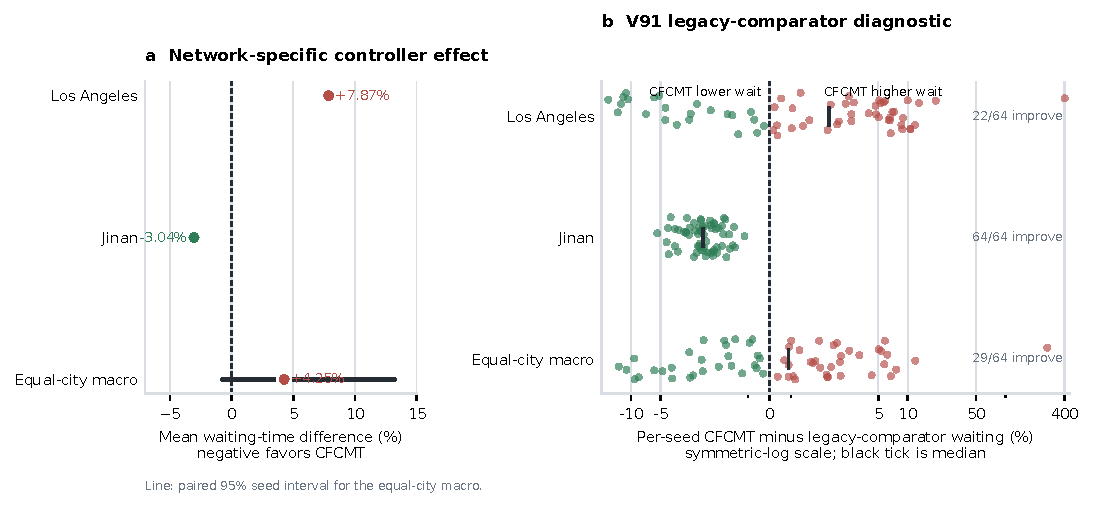
\includegraphics[width=\textwidth]{tsc_source_contribution_diagnostic.pdf}
\caption{Network dependence in the fresh V91 comparison.  \textbf{a}, Mean
all-departed waiting differences for Los Angeles, Jinan and the equal-city
primary estimand.  Negative values favour CFCMT; the line shows the paired
95\% interval for the equal-city mean. \textbf{b}, Seed-level city and equal-city
differences for all 64 fresh seeds.  Every Jinan city contrast favours CFCMT,
whereas Los Angeles contains a long regression tail.  The comparator is the
frozen legacy near-target-only arm with a retained source prior.
It therefore differs from a strict zero-source-row target estimator.}
\label{fig:source-contribution-diagnostic}
\end{figure}
\FloatBarrier

\subsection{A target-offline selector retained a Jinan-specific controller-pair gain}

After the V91 outcomes, the V98 experiment refitted target models with repaired
topology context and separate source-city components.  Five
scenario-and-seed-blocked folds evaluated seven source groups and source masses
in $\{0,0.25,0.5,0.75,1\}$.  Selection used only a balanced subset of 100 target
adaptation action groups (B100).  Failure of the offline improvement and
fold-stability gates returned the exact target-only model.  Before fresh
closed-loop evaluation, the selector returned source mass zero for Los Angeles.
It selected Hangzhou with source mass one for Jinan before its rollouts.

The selected Jinan controller was compared with a strict zero-source-row
target model on 56 further seeds.  Three demand scenarios and two policies
produced 336 completed rollouts in this confirmation.  Equal-scenario
all-departed waiting decreased by 4.527\%, with a paired-seed 95\% bootstrap
interval of 4.279--4.787\%.  All 56 seeds improved, and the two-sided paired
Wilcoxon probability was $7.55\times10^{-11}$
(\Cref{tab:jinan-conditional-source-transfer,sec:supp-v98-confirmation}).

This extension used topology-repaired models and a pressure guard shared by
both arms.  The preselected controller improved reproducibly relative to its
declared comparator under the frozen V98 protocol.  The zero-source-row target
estimator had lower capacity, so the contrast did not isolate source-row
contribution or establish superiority over PhasePressure.  V98 and V91 were
reported separately because their model and guard configurations differed.

\begin{table}[t]
\caption{Jinan-specific controller comparisons under two separate frozen
protocols.  V91 compares the original V43 controller with its legacy
near-target-only arm.  V98 compares the subsequently selected controller with
a strict zero-source-row target model of lower capacity.  Results remain
separate, and the V98 contrast measures controller-pair performance without
isolating source-row contribution.}
\label{tab:jinan-conditional-source-transfer}
\centering
\scriptsize
\resizebox{\textwidth}{!}{\begin{tabular}{@{}>{\raggedright\arraybackslash}p{0.12\textwidth}>{\raggedright\arraybackslash}p{0.17\textwidth}rrrl>{\raggedright\arraybackslash}p{0.20\textwidth}>{\raggedright\arraybackslash}p{0.17\textwidth}@{}}
\toprule
Experiment & Selection/evaluation & Seeds & Improved & Mean relative waiting difference & 95\% interval & Comparator & Guard \\
\midrule
V91 Jinan city diagnostic & frozen two-city protocol; Jinan diagnostic & 64 & 64/64 & -3.045\% & -- & final V43 legacy near-target-only & none in final V43 controller \\
V98 Jinan controller-pair confirmation & B100 target-offline preselection; fresh Jinan confirmation & 56 & 56/56 & -4.527\% & [-4.787, -4.279]\% & strict zero-source-row lower-capacity target model (causal\_target\_only\_v2) & post-V91 shared inherited Jinan pressure guard (risk\_multiplier=0.5) \\
\midrule
\multicolumn{8}{@{}p{\textwidth}@{}}{\footnotesize Negative differences favour the first-listed controller.  The V91 row is its Jinan city diagnostic and has no city-specific interval in that audit.  V98 compares a preselected controller with its declared lower-capacity zero-source-row target comparator; the two rows are not pooled, and V98 does not isolate source-row contribution.} \\
\bottomrule
\end{tabular}
}
\end{table}
\FloatBarrier

\subsection{Classical pressure remained the performance ceiling}

In the original external matrix, MaxPressure and PhasePressure achieved
141.74 and 143.62 s all-departed waiting, respectively.  They outperformed
CFCMT by 7.43 and 5.55 s, respectively, in the equal-city comparison.  Both
external cities favoured pressure control, and the descriptive intervals
excluded zero.  Pressure policies also achieved lower system vehicle-hours
and higher completion ratios than CFCMT.  The pressure reference defined the
origin of the final controller's learned action contrast.  It could select
any feasible phase without falling back to either rule.

All 56 rollouts in this matrix completed with zero recorded teleports.
Across policies, 171 raw collision events were consolidated into 13 unique
junction incidents in six rollouts.  CFCMT had zero incidents and never
exceeded its paired comparator's incident count.  The eight CFCMT rollouts
provided an incident audit, without supporting a safety-certification claim.
The metric population and incident consolidation rules are given in
\Cref{sec:supp-metric-safety}.

\subsection{A fresh-seed successor stress test did not close the pressure gap}

After V43 was frozen, a separate successor track tested a longer-horizon
latent originator with a globally rate-limited executor against PhasePressure.
On Jinan, it used a target-state-conditioned 120-s action originator, one
network-wide override at a time and a 120-s global switch cooldown.  Its results
were kept separate from the anchored all-pair controller's two-city matrix.

The legacy global executor yielded a mean relative all-departed waiting
difference of $-0.429\%$ across 54 disclosed adaptive seeds.  Its paired 95\%
interval was $[-0.818,-0.033]\%$ in this adaptive screen.  Unlimited cooldown
stays regressed by $0.104\%$, while a one-stay budget gave an inconclusive
$-0.242\%$ point estimate.  Both variants were rejected, leaving the unchanged
legacy executor for fresh confirmation.  We froze it before generating 64
new seeds, disjoint from all adaptive seeds and eight still-sealed prospective
seeds.

On the 64 fresh seeds, the method--PhasePressure difference shrank to
$-0.043\%$ (paired 95\% interval $[-0.449,0.370]\%$).  The method improved
34/64 seeds; the one-sided exact sign-test probability was 0.354.  The worst
seed regressed by 5.21\%, exceeding the preregistered 5\% limit.  Teleports were
0/0 and collision incidents 1/1, while the bootstrap, sign-test and worst-seed
gates failed.  The joint confirmation was therefore rejected
(\Cref{sec:supp-postfreeze-stress,tab:postfreeze-stress}), leaving no confirmed
superiority over PhasePressure on Jinan or across networks.

\subsection{Native RL experiments verified baseline execution}

Official RESCO and patched LibSignal experiments verified the execution of
standard RL baselines.  The RESCO adapter completed 42 supported full-budget
runs under its native protocol.  The LibSignal adapter completed 36 runs across
deep Q-network (DQN), its independent variant (IDQN), PressLight, FRAP and
MPLight.  These runs retained native observations, rewards, action intervals,
training loops and metrics.  Their distinct protocols excluded them from the
paired 56-rollout comparison above.  Results and upstream exclusions are
reported in \Cref{sec:supp-native-rl,tab:official-resco-rl,tab:libsignal-rl}.

\FloatBarrier
